\section{The MMT System, the OpenDreamKit project, and The Math-In-The-Middle approach}\label{sec:mmtmitm}

We start by giving the reader an overview of the underlying of the \omdocmmt\ theory graphs. 
This is a flexiformal representation of mathematical knowledge, which is represented in the the \omdocmmt language, mechanized by the MMT system, and stored in the MathHub information system. 

\mmt\ \cite{Rabe:MMTLanguageSystem09} is a language and framework that was developed to manage (mainly) mathematical knowledge. 
It can handle both formal and informal content. 
\mmt\ is under active development and the project home page can be found at \cite{uniformal:on}. 

\subsection{Knowledge Representation In \omdocmmt}\label{sec:mmtmitm:kr}

Knowledge inside of \mmt\ employs the theory graph paradigm supported by the underlying \omdocmmt\ language. 
This means that knowledge is organized in distinct theories which are related by different relations in a graph-like manner. 
One of these relations is a so-called view, which can be used to translate knowledge from one theory to another. 
Definiens within each theory are identified by a URI (the so-called \mmt\ URI) whereas the definitions are represented by what amounts to OpenMath \cite{BusCapCar:oms04} objects. 
Apart from making purely formal declarations, it is also possible to annotate the declarations with human-readable, narrative elements. 

Commonly all knowledge in \mmt\ is manifested on disk and loaded by the system in its entirety on startup. 
This means that there is a set of files, specifically XML files, on disk containing the appropriate theories and declarations. 
We refer to theories stored in this form as \textit{concrete theories}. 

Knowledge in \mmt\ can be accessed by either giving it's name -- i.e. it's \mmt\ URI, 
or by giving a set of conditions that has to fulfilled by the knowledge in question. 
The achieve the latter, \mmt\ has a Query Language called QMT, which allows even complex conditions to be specified. 

This modeling of mathematical knowledge has proven very effective. 
On top of pure mathematical knowledge modeling, it is also possible to annotate declarations. 
This means one can give them human-readable descriptions.
The other direction, giving informal knowledge (for example a paper) a partially formal meaning is also possible.

This has allowed us to develop and populate a system called MathHub \cite{MathHub:on}. 
The system altogether forms a big theory graph totaling at about 10000 theories. 
MathHub is far more than just a theory graph however, it allows creating and editing of existing libraries and offers possibilities for integrating semantic services.
The deatils of this are not relevant to the topic at hand -- we refer the interested reader to \cite{Iancu:phd} instead.

Notable projects available on MathHub include SMGloM \cite{SMGloM:on} -- a semantic glossary of mathematical knowledge -- LATIN \cite{LATIN:online} -- a logical atlas of several different formalizations  -- as well as parts of the PVS \cite{PVSlibraries:on}, MiZar \cite{mizar:online} and HOL Light \cite{KalRab:hollight:14} libraries.

\subsection{Virtual Theories In The Math-In-The-Middle approach}\label{sec:mmtmitm:odk}

The OpenDreamKit \cite{OpenDreamKit:on} project is an EU-funded project that aims to create Virtual Research Environments enabling mathematicians to make efficient use of existing Open-Source mathematical knowledge systems. 
These systems include Sage, GAP and \lmfdb\ systems, along with others. 

Aiming to create such environments, as part of the OpenDreamKit project it is necessary for the different systems to interoperate. 
Similar to the Mathematical Knowledge Bases problem here, the State-Of-The-Art of such system interaction is basically non-existent: 
Connections between different systems only exist on an ad-hoc, system-specific basis. 
These interactions both require significant work to maintain, and result in a large number of one-to-one system connections. 

\begin{wrapfigure}{l}{0.3\textwidth}
  \begin{center}
    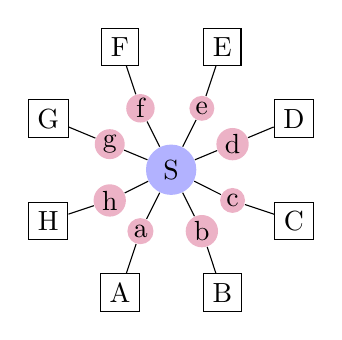
\begin{tikzpicture}[xscale=1.3,yscale=1.3]\normalsize
      \tikzstyle{withshadow}=[draw,drop shadow={opacity=.5},fill=white]
      \tikzstyle{system}=[draw]
      \tikzstyle{standard}=[circle,fill=blue!30]
      \tikzstyle{interface}=[circle,fill=purple!30,inner sep = 1pt,]
      \node[system] (a) at (0,.3) {A};
      \node[system] (b) at (1,.3) {B};
      \node[system] (c) at (1.7,1) {C};
      \node[system] (d) at (1.7,2) {D};
      \node[system] (e) at (1,2.7) {E};
      \node[system] (f) at (0,2.7) {F};
      \node[system] (g) at (-.7,2) {G};
      \node[system] (h) at (-.7,1) {H};
      \node[standard] (m) at (.5,1.5) {S};
      \node[interface] (ia) at (0.2,.9) {a};
      \node[interface] (ib) at (.8,.9) {b};
      \node[interface] (ic) at (1.1,1.2) {c};
      \node[interface] (id) at (1.1,1.75) {d};
      \node[interface] (ie) at (.8,2.1) {e};
      \node[interface] (if) at (0.2,2.1) {f};
      \node[interface] (ig) at (-.1,1.75) {g};
      \node[interface] (ih) at (-.1,1.2) {h};
      \draw (m) -- (ia) -- (a);
      \draw (m) -- (ib) -- (b);
      \draw (m) -- (ic) -- (c);
      \draw (m) -- (id) -- (d);
      \draw (m) -- (ie) -- (e);
      \draw (m) -- (if) -- (f);
      \draw (m) -- (ig) -- (g);
      \draw (m) -- (ih) -- (h);
      \end{tikzpicture}
  \end{center}

  \caption[The MITM Approach to Connecting Systems]{
    The MiTM Approach to Connecting Systems. 
  }
  \label{fig:mitmconnect}
\end{wrapfigure}
To address these problems, we have introduced the Math-In-The-Middle approach, which is illustrated in Figure~\ref{fig:mitmconnect}. 
It models the true, underlying mathematical semantics in \mmt\ and allows translation between this centrally formalized knowledge and the systems on the boundary.
This mathematical knowledge is modeled using the well-established theory graph paradigm and is stored inside our MathHub / \mmt\ architecture. 

The knowledge in the systems themselves is also modeled via theories in a theory graph.
This allows us to implement translation with the help of bi-views -- views in both directions -- between the central knowledge -- the Math-In-The-Middle -- and each of the systems. 

As part of this approach, the integrated systems include the systems of the OpenDreamKit project, along with several Mathematical Knowledge Bases. 
Within this approach, the knowledge in these has to be modelled using a theory graph. 
Here we have made of Virtual Theories. 

In a nutshell, virtual theories are just like concrete theories, but without the assumption of loading all declarations from a file on disk at system startup. 
Instead of loading all knowledge from an XML file, virtual theories load declarations in a lazy fashion when they are required. 
Here we do not even restrict ourselves to lazily reading an XML file, on the contrary, in most use cases we actually create the \omdocmmt\ representation on demand. 

We will not go into much detail more detail of either the OpenDreamKit project, or the Math-In-The-Middle approach as a whole here. 
Instead, we will focus only on Virtual Theories. 
We refer the interested reader to \ednote{Cite MACIS17-interop}, a paper submitted by a superset of the authors of this paper, describing the approach in detail. 

%%% Local Variables:
%%% mode: latex
%%% TeX-master: "paper"
%%% End:

%  LocalWords:  omdocmmt fig:classicalconnect fig:mitmconnect OpenDreamKit:on lmfdb lmfdb
%  LocalWords:  ODKproposal:on DehKohKon:iop16 sagemath oeis fig:mitmontology colored
%  LocalWords:  mathrm mathrm
